%package list
\documentclass{article}
\usepackage[top=3cm, bottom=3cm, outer=3cm, inner=3cm]{geometry}
\usepackage{multicol}
\usepackage{graphicx}
\usepackage{url}
%\usepackage{cite}
\usepackage{hyperref}
\usepackage{array}
%\usepackage{multicol}
\newcolumntype{x}[1]{>{\centering\arraybackslash\hspace{0pt}}p{#1}}
\usepackage{natbib}
\usepackage{pdfpages}
\usepackage{multirow}
\usepackage[normalem]{ulem}
\useunder{\uline}{\ul}{}
\usepackage{svg}
\usepackage{xcolor}
\usepackage{listings}

\lstdefinestyle{ascii-tree}{
    literate={├}{|}1 {─}{--}1 {└}{+}1 
  }
\lstset{basicstyle=\ttfamily,
  showstringspaces=false,
  commentstyle=\color{red},
  keywordstyle=\color{blue}
}
%\usepackage{booktabs}
\usepackage{caption}
\usepackage{subcaption}
\usepackage{float}
\usepackage{array}

\newcolumntype{M}[1]{>{\centering\arraybackslash}m{#1}}
\newcolumntype{N}{@{}m{0pt}@{}}


%%%%%%%%%%%%%%%%%%%%%%%%%%%%%%%%%%%%%%%%%%%%%%%%%%%%%%%%%%%%%%%%%%%%%%%%%%%%
%%%%%%%%%%%%%%%%%%%%%%%%%%%%%%%%%%%%%%%%%%%%%%%%%%%%%%%%%%%%%%%%%%%%%%%%%%%%
\newcommand{\itemEmail}{kllacma@unsa.edu.pe}
\newcommand{\itemStudent}{Kevin Andree Llacma Quispe}
\newcommand{\itemCourse}{Programacion web 2}
\newcommand{\itemCourseCode}{20200585}
\newcommand{\itemSemester}{I}
\newcommand{\itemUniversity}{Universidad Nacional de San Agustín de Arequipa}
\newcommand{\itemFaculty}{Facultad de Ingeniería de Producción y Servicios}
\newcommand{\itemDepartment}{Departamento Académico de Ingeniería de Sistemas e Informática}
\newcommand{\itemSchool}{Escuela Profesional de Ingeniería de Sistemas}
\newcommand{\itemAcademic}{2024 - A}
\newcommand{\itemInput}{-}
\newcommand{\itemOutput}{-}
\newcommand{\itemPracticeNumber}{02}
\newcommand{\itemTheme}{Git Docker}
%%%%%%%%%%%%%%%%%%%%%%%%%%%%%%%%%%%%%%%%%%%%%%%%%%%%%%%%%%%%%%%%%%%%%%%%%%%%
%%%%%%%%%%%%%%%%%%%%%%%%%%%%%%%%%%%%%%%%%%%%%%%%%%%%%%%%%%%%%%%%%%%%%%%%%%%%

\usepackage[english,spanish]{babel}
\usepackage[utf8]{inputenc}
\AtBeginDocument{\selectlanguage{spanish}}
\renewcommand{\figurename}{Figura}
\renewcommand{\refname}{Referencias}
\renewcommand{\tablename}{Tabla} %esto no funciona cuando se usa babel
\AtBeginDocument{%
	\renewcommand\tablename{Tabla}
}

\usepackage{fancyhdr}
\pagestyle{fancy}
\fancyhf{}
\setlength{\headheight}{30pt}
\renewcommand{\headrulewidth}{1pt}
\renewcommand{\footrulewidth}{1pt}
\fancyhead[L]{\raisebox{-0.2\height}{
\includegraphics[width=3cm]{img/logo_episunsa.png}}}
\fancyhead[C]{\fontsize{7}{7}\selectfont	\itemUniversity \\ \itemFaculty \\ \itemDepartment \\ \itemSchool \\ \textbf{\itemCourse}}
\fancyhead[R]{\raisebox{-0.2\height}{
\includegraphics[width=1.2cm]{img/logo_abet}}}
\fancyfoot[L]{Estudiante Kevin Llacma}
\fancyfoot[C]{\itemCourse}
\fancyfoot[R]{Página \thepage}

% para el codigo fuente

\usepackage{listings}
\usepackage{color, colortbl}
\definecolor{dkgreen}{rgb}{0,0.6,0}
\definecolor{gray}{rgb}{0.5,0.5,0.5}
\definecolor{mauve}{rgb}{0.58,0,0.82}
\definecolor{codebackground}{rgb}{0.95, 0.95, 0.92}
\definecolor{tablebackground}{rgb}{0.8, 0, 0}

\lstset{frame=tb,
	language=bash,
	aboveskip=3mm,
	belowskip=3mm,
	showstringspaces=false,
	columns=flexible,
	basicstyle={\small\ttfamily},
	numbers=none,
	numberstyle=\tiny\color{gray},
	keywordstyle=\color{blue},
	commentstyle=\color{dkgreen},
	stringstyle=\color{mauve},
	breaklines=true,
	breakatwhitespace=true,
	tabsize=3,
	backgroundcolor= \color{codebackground},
}

\begin{document}
	
	\vspace*{10px}
	
	\begin{center}	
		\fontsize{17}{17} \textbf{ Informe de Laboratorio \itemPracticeNumber}
	\end{center}
	\centerline{\textbf{\Large Tema: \itemTheme}}
	%\vspace*{0.5cm}	

	\begin{flushright}
		\begin{tabular}{|M{2.5cm}|N|}
			\hline 
			\rowcolor{tablebackground}
			\color{white} \textbf{Nota}  \\
			\hline 
			     \\[30pt]
			\hline 			
		\end{tabular}
	\end{flushright}	

	\begin{table}[H]
		\begin{tabular}{|x{4.7cm}|x{4.8cm}|x{4.8cm}|}
			\hline 
			\rowcolor{tablebackground}
			\color{white} \textbf{Estudiante} & \color{white}\textbf{Escuela}  & \color{white}\textbf{Asignatura}   \\
			\hline 
			{\itemStudent \par \itemEmail} & \itemSchool & {\itemCourse \par Semestre: \itemSemester \par Código: \itemCourseCode}     \\
			\hline 			
		\end{tabular}
	\end{table}		
	
	\begin{table}[H]
		\begin{tabular}{|x{4.7cm}|x{4.8cm}|x{4.8cm}|}
			\hline 
			\rowcolor{tablebackground}
			\color{white}\textbf{Laboratorio} & \color{white}\textbf{Tema}  & \color{white}\textbf{Duración}   \\
			\hline 
			\itemPracticeNumber & \itemTheme & 04 horas   \\
			\hline 
		\end{tabular}
	\end{table}
	
	\begin{table}[H]
		\begin{tabular}{|x{4.7cm}|x{4.8cm}|x{4.8cm}|}
			\hline 
			\rowcolor{tablebackground}
			\color{white}\textbf{Semestre académico} & \color{white}\textbf{Fecha de inicio}  & \color{white}\textbf{Fecha de entrega}   \\
			\hline 
			\itemAcademic & \itemInput &  \itemOutput  \\
			\hline 
		\end{tabular}
	\end{table}
\title{Programación Web\\Laboratorio 02\\Tema: Git y GitHub}

\maketitle

\section{Especificaciones del Laboratorio}
\subsection{Objetivos del curso}
\begin{itemize}
    \item Proporcionar los conocimientos y habilidades para el uso de las principales metodologías de análisis y diseño de sistemas.
    \item Brindar los conocimientos para la utilización de técnicas para el análisis y diseño de sistemas web.
    \item Proporcionar conocimientos y habilidades en el manejo de herramientas para el desarrollo de sistemas Web.
    \item Desarrollar sistemas de información dentro de una arquitectura cliente servidor.
\end{itemize}

\subsection{Objetivos del laboratorio}
\begin{itemize}
    \item Utilizar el sistema de control de versiones Git.
    \item Utilizar la plataforma GitHub para replicar y administrar proyectos de programación.
\end{itemize}

\subsection{Equipos, materiales y temas}
\begin{itemize}
    \item Sistema Operativo (GNU/Linux de preferencia).
    \item Editor de texto plano (GNU Vim de preferencia).
    \item Navegador Web: Chrome, Firefox, Edge, Brave, Opera, etc.
    \item Git.
    \item Cuenta en GitHub asociada al correo institucional.
\end{itemize}

\section{Marco teórico}
\subsection{PowerShell}
PowerShell es una solución de automatización de tareas multiplataforma compuesta por un shell de línea de comandos, un lenguaje de secuencias de comandos y un marco de gestión de configuración. PowerShell se ejecuta en Windows, Linux y macOS.

\subsection{La W3C y los Estándares Web}
El World Wide Web Consortium o simplementa la W3C, desarrolla estándares y pautas para ayudar a todos a construir una web basada en los principios de accesibilidad , internacionalización , privacidad y seguridad.

Los estándares web son planos, o bloques de construcción, de un mundo conectado digitalmente consistente y armonioso. Se implementan en navegadores, blogs, motores de búsqueda y otro software que potencia nuestra experiencia en la web.



\subsection{Vim}
Vim es un editor de texto altamente configurable creado para hacer que la creación y el cambio de cualquier tipo de texto sean muy eficientes. Se incluye como "viçon la mayoría de los sistemas UNIX y con Apple OS X.

Vim es muy estable y se desarrolla continuamente para mejorar aún más. Entre sus características se encuentran:
\begin{itemize}
    \item árbol de deshacer persistente de varios niveles
    \item amplio sistema de complementos
    \item soporte para cientos de lenguajes de programación y formatos de archivo
    \item poderosa búsqueda y reemplazo
    \item se integra con muchas herramientas
\end{itemize}


\begin{lstlisting}[language=bash]
$ sudo apt-get install vim  # Vim en GNU/Linux
$ brew install macvim  # Vim en MacOSX
\end{lstlisting}

\subsection{Visual Studio Code}
Visual Studio Code es un editor de código fuente ligero pero potente que se ejecuta en su escritorio y está disponible para Windows, macOS y Linux. Viene con soporte integrado para JavaScript, TypeScript y Node.js y tiene un rico ecosistema de extensiones para otros lenguajes y tiempos de ejecución (como C++, C, Java, Python, PHP, Go, .NET).

Videotutoriales: \url{https://code.visualstudio.com/docs/getstarted/introvideos}

Descarga: \url{https://code.visualstudio.com/Download}

\subsection{Git}
Git es un sistema de control de versiones distribuido gratuito y de código abierto diseñado para manejar todo, desde proyectos pequeños hasta proyectos muy grandes, con rapidez y eficiencia.

Documentación: \url{https://git-scm.com/doc}

Descargas: \url{https://git-scm.com/downloads}

\subsection{GitHub}
GitHub es una plataforma de hospedaje de código para el control de versiones y la colaboración. Este permite que tú y otras personas trabajen juntos en proyectos desde donde sea.

Documentación: \url{https://docs.github.com/es}

\subsection{Arquitectura Git}


Git tiene tres estados principales en los que se pueden encontrar tus archivos: confirmado (committed), modificado (modified), y preparado (staged).
\begin{itemize}
    \item Confirmado: significa que los datos están almacenados de manera segura en tu base de datos local.
    \item Modificado: significa que has modificado el archivo pero todavía no lo has confirmado a tu base de datos.
    \item Preparado: significa que has marcado un archivo modificado en su versión actual para que vaya en tu próxima confirmación.
\end{itemize}

Esto nos lleva a las tres secciones principales de un proyecto de Git: El directorio de Git (Git directory), el directorio de trabajo (working directory), y el área de preparación (staging area).

\subsection{Estándares de codificación}
Los estándares de código son una serie de reglas definidas para un lenguaje de programación, o bien, un estilo de programación específico.

El estilo garantiza que todos los ingenieros que contribuyen a un proyecto tengan una forma única de diseñar su código, lo que da como resultado una base de código coherente, asegurando una fácil lectura y mantenimiento.

El uso de estándares es muy importante en la calidad de software, sin embargo mantener todos los proyectos cumpliendo a la perfección con esto no es una tarea fácil, requiere un gran esfuerzo y constancia por parte del equipo de desarrollo.

Mientras más y más compañías han adoptado estándares, todavía hay aquellas que realizan el desarrollo de sus proyectos sin ellos.


\section{Desarollo del lab}
Primero se instalo el docker a windows
Para lograr correr una pagina web con docker contenedores:
Se crea el archivo "Dockerfile" donde colocamos:
    \begin{figure}[H]
		          \centering
		          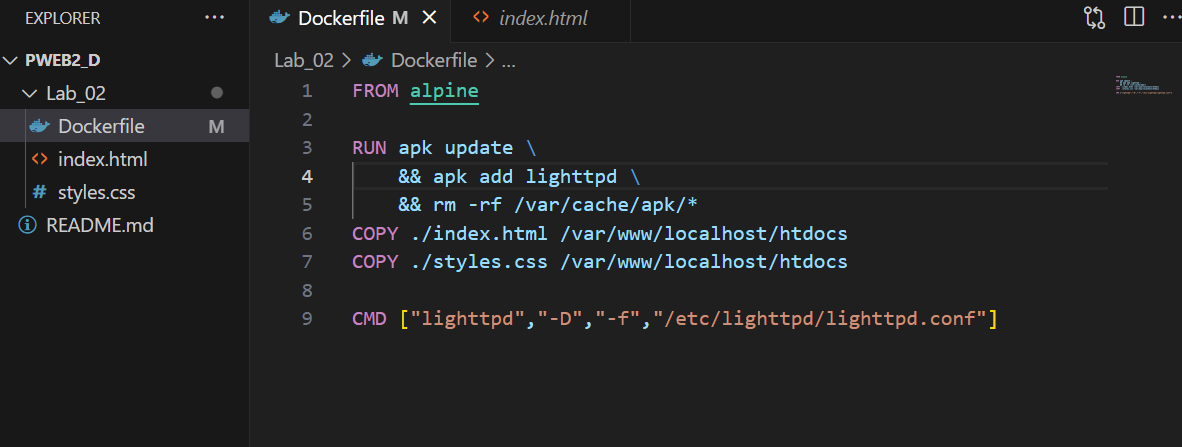
\includegraphics[width=0.8\textwidth,keepaspectratio]                       {img/Dockerfile_alpine.png}
		             %\includesvg{img/automata.svg}
		              %\label{img:mot2}
		              %\caption{Product backlog.}
    \end{figure}
Seguido se uso un archivo "index.html" con sus estilos para que pueda usarlos
    \begin{figure}[H]
		          \centering
		          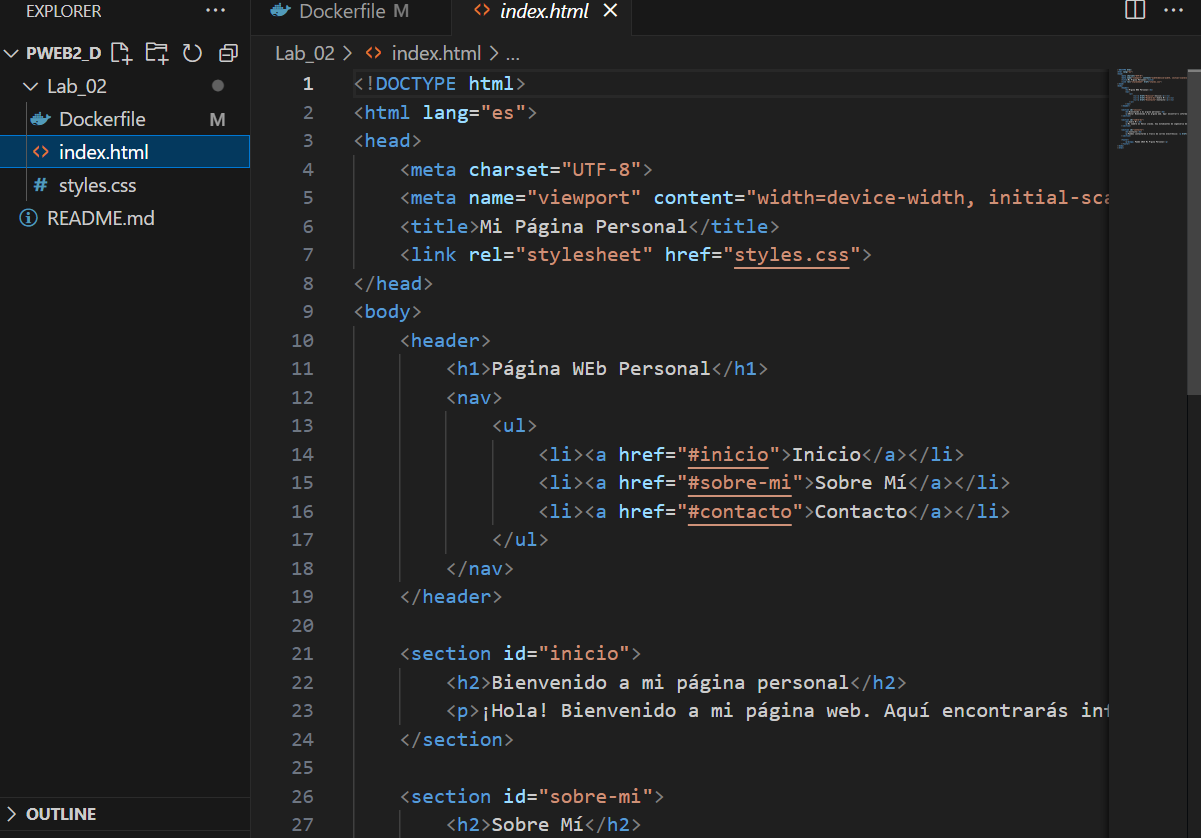
\includegraphics[width=0.8\textwidth,keepaspectratio]                       {img/index_html.png}
		             %\includesvg{img/automata.svg}
		              %\label{img:mot2}
		              %\caption{Product backlog.}
    \end{figure}
Ahora usamos docker build para crear una imagen Docker esto usando el archivo Dockerfile
     \begin{figure}[H]
		          \centering
		          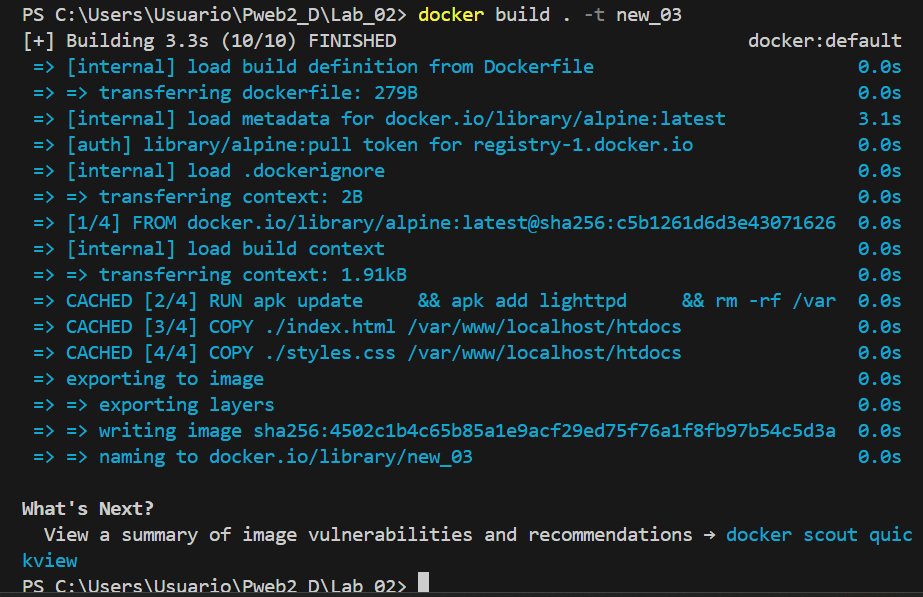
\includegraphics[width=0.8\textwidth,keepaspectratio]                       {img/Docker_build.png}
		             %\includesvg{img/automata.svg}
		              %\label{img:mot2}
		              %\caption{Product backlog.}
    \end{figure}

Se uso el comando Docker run para crear y ejecutar un contenedor Docker a partir de una imagen Docker existente.
    \begin{figure}[H]
		          \centering
		          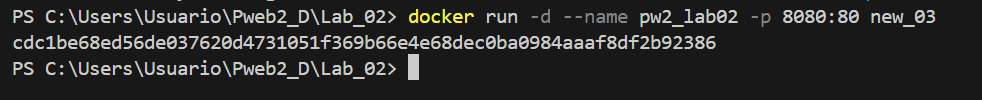
\includegraphics[width=0.8\textwidth,keepaspectratio]                       {img/Docker_run.png}
		             %\includesvg{img/automata.svg}
		              %\label{img:mot2}
		              %\caption{Product backlog.}
    \end{figure}
Al ejecutar el comando podemos ver que en docker desktop aparece el contenedor que esta ejecuntandose
    \begin{figure}[H]
		          \centering
		          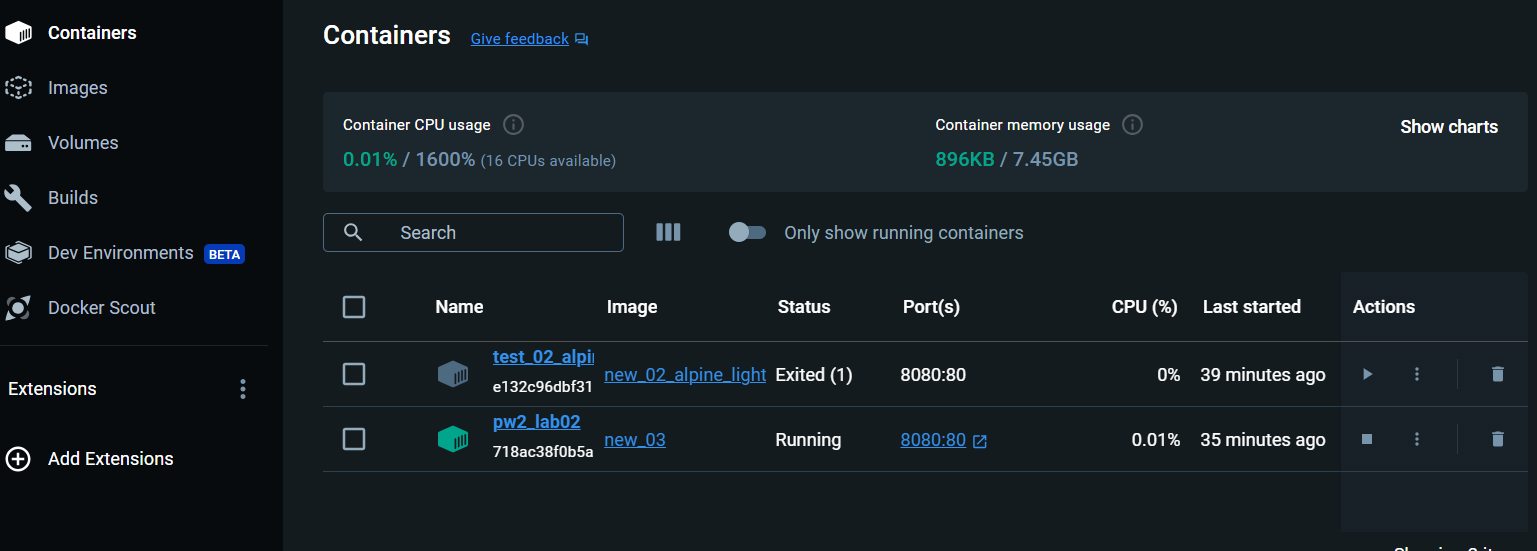
\includegraphics[width=0.8\textwidth,keepaspectratio]                       {img/Docker_desktop.png}
		             %\includesvg{img/automata.svg}
		              %\label{img:mot2}
		              %\caption{Product backlog.}
    \end{figure}
Ahora podemos ver en el puerto 8080 que esta corriendo la pagina a travez de docker

    \begin{figure}[H]
		          \centering
		          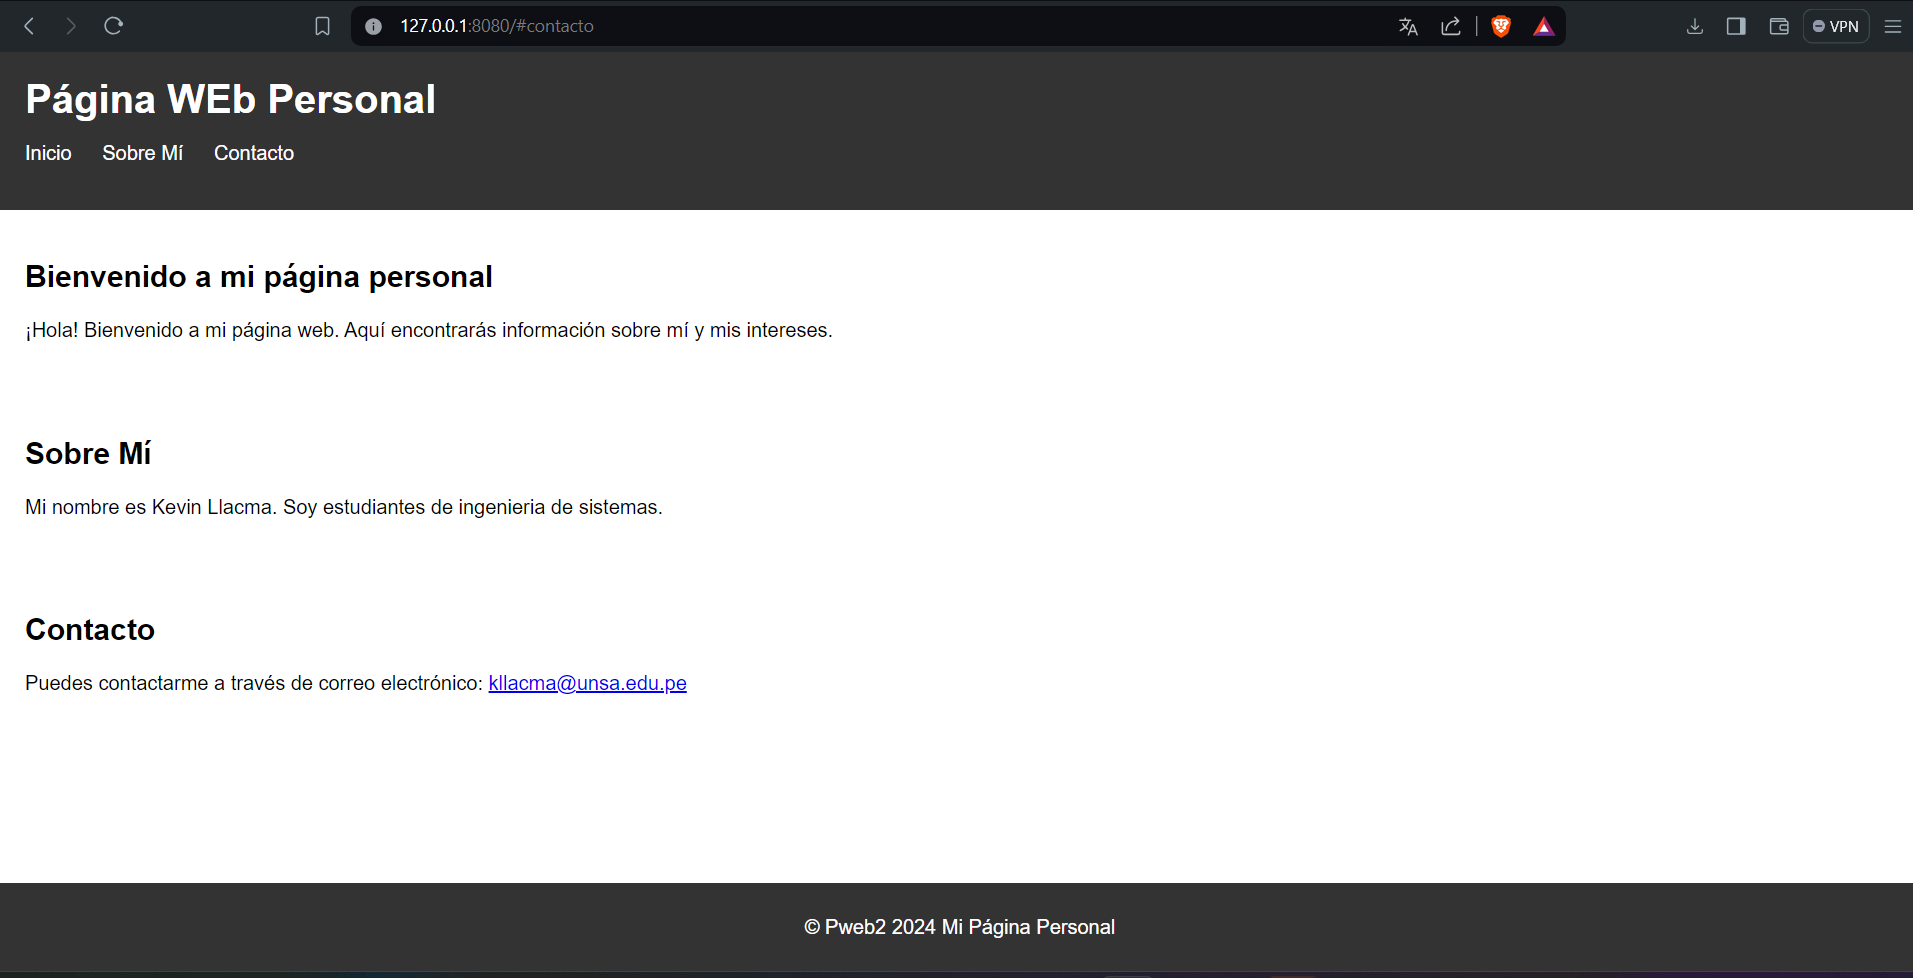
\includegraphics[width=0.8\textwidth,keepaspectratio]                       {img/pagina_corriendo.png}
		             %\includesvg{img/automata.svg}
		              %\label{img:mot2}
		              %\caption{Product backlog.}
    \end{figure}

\end{document}